\documentclass[a4paper,11pt]{article}
% !TeX program = pdflatex
\pdfoutput=1
\pdfminorversion=7
\usepackage[utf8]{inputenc}
\usepackage{CJKutf8}
\AtBeginDocument{\begin{CJK*}{UTF8}{gbsn}}
\AtEndDocument{\clearpage\end{CJK*}}
\usepackage{jheppub}

\usepackage{amsmath,amssymb,latexsym}
\usepackage{braket}
\usepackage{bm}
\usepackage{booktabs}
\usepackage{tabularx}
\usepackage{cancel}
\usepackage[svgnames]{xcolor}
\usepackage{hepunits}
\usepackage{mathtools}
\usepackage{graphicx}
\usepackage[most]{tcolorbox}
\usepackage{caption}
\usepackage{tikz}
\usetikzlibrary{calc}
\def\ie{\begin{equation}\begin{aligned}}
\def\fe{\end{aligned}\end{equation}}
\newtcolorbox{proofbox}{
  enhanced, breakable, colback=gray!8, colframe=black,
  boxrule=0.8pt, arc=0pt, outer arc=0pt,
  left=8pt, right=8pt, top=8pt, bottom=8pt,
  before skip=10pt, after skip=10pt
}
\hypersetup{colorlinks=true,linkcolor=blue,citecolor=blue,urlcolor=blue}

\title{dS IBP Package 用户手册}
\author[a]{Su Yingze}
\affiliation[a]{Institute not specified}
\emailAdd{yingze.su@outlook.com}
\abstract{本手册说明 dS IBP package 的费曼规则、统一积分表示、massive/massless 指标约定、time 与 loop-momentum IBP、独立变量微分方程 seed、EOM/缩并 canonical、拓扑输入、公开 API、Kira 接口和 tree vertex family。当前稳定主线为 015：圈线相关独立外动量使用完整 \texttt{ssij} 根号 Gram 坐标；其它实际出现的无圈动量模长平方按首次出现顺序选独立基并绑定为 \texttt{sE1,sE2,...}，从属项保存 binding，同时复用 014 的平方 Gram 原子导数；package 只生成、序列化和验证关系，不运行 reduction。}

\begin{document}
\maketitle
\tableofcontents
\newpage

\section{快速开始与当前边界}

本 package 生成 dS 圈图的 canonical IBP seed，并把关系转换为后端中立的 \texttt{linearData}。当前稳定主线为模块化 015，支持 topology-driven 的任意圈数、任意拓扑以及 massive/massless 混合内线；标准入口和单文件兼容入口分别为
\begin{verbatim}
000_code/015_dSIBP/
000_code/015_dS_ibp_general.wl
\end{verbatim}
010--014 是只读历史/基线版本。015 继承标准 context、初始化 metadata、完整 time/loop-momentum 生成元、massive EOM、massless 有向单 $n$、共同-theta odd-subset contact、contact 可达 sector、跨 sector coincident canonical、tree 迭代与 dlog、Kira serializer/importer 以及 DE/scaling 检查，并增加根号动力学坐标 adapter。

仓库内标准加载与独立 benchmark 单文件加载是两个等价入口，应在新 kernel 中任选其一：
\begin{verbatim}
packageDir = FileNameJoin[{Directory[],"000_code","015_dSIBP"}];
If[!MemberQ[$Path,packageDir],AppendTo[$Path,packageDir]];
Needs["dSIBP`"];

(* 独立 benchmark 的自包含单文件入口： *)
Get["independent-benchmark/package/package_015.wl"];
\end{verbatim}
两者都提供 \texttt{dSIBP`} 公开 context；独立交付文件不依赖主线模块路径。不要在同一 kernel 重复加载两个入口。

推荐工作流为
\begin{enumerate}
  \item 输入顶点、内线、圈/外动量基、ISP、零点和必要的数值规则；
  \item 用 \texttt{DSInit} 验证输入、ISP 坐标、函数系统与 contact-reachable sectors；
  \item 用 \texttt{DSSeeds} 生成每个 sector 的全部 time 与 loop-momentum seed；需要完整离散态时显式传 \texttt{DiscreteMode->"all"}；
  \item seed 层立即执行 EOM/symmetry/canonical，并保留 Mathematica 表达式；
  \item 用 \texttt{DSLinear} 构造后端中立 \texttt{linearData}；必要的小规模数值规则只在这一层代入；
  \item 按需调用 \texttt{DSKiraExport}；用户在 package 外运行 reduction；
  \item 有完整外部结果时用 \texttt{DSKiraImport -> DSDE -> DSScaleCheck} 取回并验证。
\end{enumerate}

\begin{proofbox}
解析 seed 只允许小规模生成。禁止默认展开整族解析 IBP，也禁止为了验证做宽范围撒点。所有 WolframScript 检查必须显示消息运行，不能用 \texttt{Quiet} 掩盖问题。
\end{proofbox}

给定下文的 \texttt{case} 后，最短的可执行调用链是
\begin{verbatim}
context = DSInit[case];
seeds = DSSeeds[
  context,
  DiscreteMode -> "all",
  GenerateShrinkSectors -> True
];
linearData = DSLinear[seeds,context];
{context["status"],seeds["dSIBPStatus"],
 linearData["dSIBPStatus"]}
\end{verbatim}
每个批量接口都返回 Association；必须先检查 \texttt{"status"}，再读取方程或传给下一阶段。

独立 benchmark 的 \texttt{package/examples/} 提供六个应用例子：
\begin{verbatim}
01_mixed_bubble_workflow.wl
02_function_system_hankel.wl
03_two_loop_isp.wl
04_pure_massive_bubble_closed_loop/main.wl
05_tree_two_vertex_time_ibp/main.wl
06_root_kinematic_coordinates/main.wl
\end{verbatim}
它们分别展示 mixed massive/massless 工作流、一般 \texttt{P,Q,T,W} 函数系统、两圈 ISP、pure massive bubble 的外部 Kira 闭环、两顶点 tree pure-time/dlog 路线，以及 015 的 \texttt{ssij/sEe} 初始化与总导数。examples 不含独立 expected；Kira example 只写输入并取回已有结果，不启动 reduction。

\section{SK 费曼规则到积分族}

\subsection{顶点规则}

每个时间顶点 $v$ 有共形时间 $\tau_v<0$ 和 SK 分支 $\sigma_v=\pm$。本 package 使用
\begin{equation}
  \sigma_v=+:\quad e^{-iE_v\tau_v},
  \qquad
  \sigma_v=-:\quad e^{+iE_v\tau_v}.
\end{equation}
因此外腿相位对 time-IBP 的贡献为
\begin{equation}
  \partial_{\tau_v}e^{-iE_v\tau_v}=-iE_v e^{-iE_v\tau_v},
  \qquad
  \partial_{\tau_v}e^{+iE_v\tau_v}=+iE_v e^{+iE_v\tau_v}.
  \label{vertexPhaseRule}
\end{equation}
$E_v$ 表示连接该顶点的所有外腿模长在指数中形成的打包能量。它不一定是进入圈内线动量的外部向量。

\subsection{内线的四种类型}

设内线 $e$ 的有序端点为 $\{u_e,v_e\}$，动量为
\begin{equation}
 \bm Q_e=\sum_{\ell=1}^{L}c_{e\ell}\bm q_\ell
        +\sum_{j=1}^{K}d_{ej}\bm k_j,
 \qquad q_e=|\bm Q_e|.
\end{equation}
端点的 SK 符号决定传播子类型：
\begin{center}
\begin{tabular}{lll}
\toprule
质量类型 & 端点分支 & 指标包\\
\midrule
massive & 同分支 $++/--$ & \texttt{\{b[e],n[e,1],n[e,2]\}}\\
massive & 异分支 $+-/-+$ & \texttt{\{b[e],n[e,1],n[e,2]\}}\\
massless & 同分支 $++/--$ & \texttt{\{b[e],n[e]\}}\\
massless & 异分支 $+-/-+$ & \texttt{\{b[e]\}}\\
\bottomrule
\end{tabular}
\end{center}
同分支线含 theta ordering，称为 full line；异分支线没有 theta 导数产生的 shrink，称为 cross line。massive cross 仍有两个 Hankel 端点态；massless cross 是单个指数乘积，因此没有离散 $n$。

\subsection{Bubble 图作为输入例子}

下图只是一个 topology 输入例子，不代表生成器硬编码 bubble。两条内线可分别选为 massive/massless full/cross；只需改变 family metadata，统一积分 Head 不变。

\begin{center}
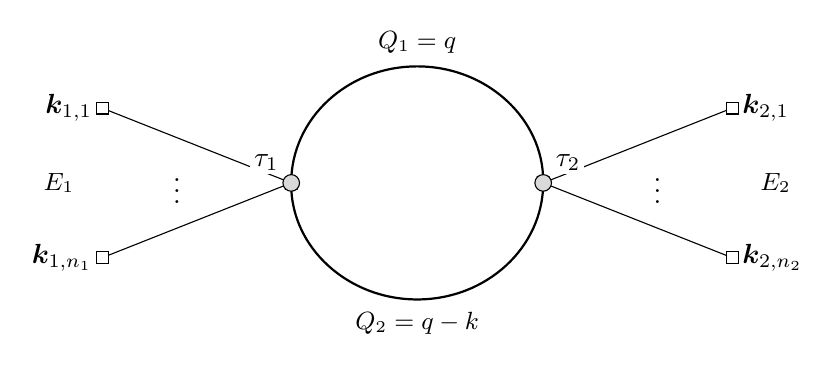
\begin{tikzpicture}[scale=1.0, every node/.style={inner sep=1.5pt}]
  \coordinate (vL) at (0,0);
  \coordinate (vR) at (3.2,0);
  \coordinate (lU) at (-2.4,0.95);
  \coordinate (lD) at (-2.4,-0.95);
  \coordinate (rU) at (5.6,0.95);
  \coordinate (rD) at (5.6,-0.95);
  \draw (vL) -- (lU) node[left=2pt] {$\bm{k}_{1,1}$};
  \draw (vL) -- (lD) node[left=2pt] {$\bm{k}_{1,n_1}$};
  \draw (vR) -- (rU) node[right=2pt] {$\bm{k}_{2,1}$};
  \draw (vR) -- (rD) node[right=2pt] {$\bm{k}_{2,n_2}$};
  \node[fill=white,inner sep=1pt] at (-1.45,0) {$\vdots$};
  \node[fill=white,inner sep=1pt] at (4.65,0) {$\vdots$};
  \draw[->,thick] (vL) arc[start angle=180,end angle=0,x radius=1.6,y radius=1.48];
  \draw[->,thick] (vR) arc[start angle=0,end angle=-180,x radius=1.6,y radius=1.48];
  \node[fill=white] at (1.6,1.78) {\small $Q_1=q$};
  \node[fill=white] at (1.6,-1.78) {\small $Q_2=q-k$};
  \node[fill=white] at (-2.95,0) {\small $E_1$};
  \node[fill=white] at (6.15,0) {\small $E_2$};
  \filldraw[fill=gray!30,draw=black] (vL) circle (3pt);
  \filldraw[fill=gray!30,draw=black] (vR) circle (3pt);
  \node[fill=white,anchor=south east] at (-0.10,0.10) {$\tau_1$};
  \node[fill=white,anchor=south west] at (3.30,0.10) {$\tau_2$};
  \filldraw[fill=white,draw=black] ($(lU)+(-0.075,0.075)$) rectangle ++(0.15,-0.15);
  \filldraw[fill=white,draw=black] ($(lD)+(-0.075,0.075)$) rectangle ++(0.15,-0.15);
  \filldraw[fill=white,draw=black] ($(rU)+(-0.075,0.075)$) rectangle ++(0.15,-0.15);
  \filldraw[fill=white,draw=black] ($(rD)+(-0.075,0.075)$) rectangle ++(0.15,-0.15);
\end{tikzpicture}
\end{center}

例如 mixed bubble 可取 $Q_1=q$ 为 massive，$Q_2=q-k$ 为 massless。pure massless bubble 则把两线都设为 massless。顶点符号从 $++$ 改成 $+-$ 时，两条线自动从 full 变为 cross；不是换一套积分 Head。

\section{统一三槽积分表示}

所有 top/sub-sector 都使用三个正式槽位
\begin{equation}
 \boxed{
 J\!\left[
   \{a_v\},
   \{\mathrm{pack}_e\},
   \{n_{\mathrm{isp},r}\}
 \right]}
 \equiv
 \texttt{J[aList,linePacks,ispList]}.
 \label{threeSlotJ}
\end{equation}
三个槽位分别是
\begin{enumerate}
  \item \texttt{aList}：当前 sector 的独立时间变量幂次；
  \item \texttt{linePacks}：按固定 line slot 排列的传播子/缩并线指标包；
  \item \texttt{ispList}：ISP 的正式指标槽，不是附注 metadata。
\end{enumerate}

实际幂次包含初始化零点：
\begin{equation}
 A_v=a_v+a0_v,\qquad
 B_e=b_e+b0_e,\qquad
 B^S_e=bS_e+bS0_e.
\end{equation}
质量、$\nu_e$、端点、SK 符号、动量表达式、顶点能量、外不变量名称和 symmetry rules 都不写入 $J$。

theta 导数缩并线时，pack 变为
\begin{equation}
  \mathrm{pack}_e=\{bS_e\}.
\end{equation}
delta 函数合并两个时间变量，所以 \texttt{aList} 只保留一个代表顶点槽；原顶点到 compact slot 的映射保存在 \texttt{sectorMetadataList}。line slot 始终保留，不能删除 $bS_e$。

\section{Massive 导数、EOM 与缩并}

\subsection{端点导数与即时 EOM}

massive full/cross 的两个端点态均取 $n_{e,r}=0,1$。time 导数先产生
\begin{equation}
 \partial_{\tau_r}:\qquad
 -J[\ldots,\{b_e-1,n_{e,r}+1,\ldots\},\ldots].
\end{equation}
若 $n_{e,r}=1$，二阶态必须立刻 EOM。对 h：
\begin{equation}
 J[n_{e,r}=2]
 =-J[n_{e,r}=0]
  -(2\nu_e+1)J[a_r-1,b_e+1,n_{e,r}=1].
 \label{massiveEOM}
\end{equation}
对裸 H：
\begin{equation}
 J_H[n_{e,r}=2]
 =-J_H[n_{e,r}=0]
  -J_H[a_r-1,b_e+1,n_{e,r}=1]
  +\nu_e^2J_H[a_r-2,b_e+2,n_{e,r}=0].
 \label{bareHEOM}
\end{equation}
另一端点指标不变。最后一项就是 $\nu_e^2/x^2$ 二次 pole；loop-momentum 导数若产生 $n=2$，同样在 seed 层立即使用对应 EOM。当前 014 由统一函数系统编译这些递推；旧版内置公式只作为历史基线。

\subsection{通用 $2\times2$ 函数系统输入}

当前 015 对每条 massive line 输入
\begin{equation}
 f''+P(x)f'+Q(x)f=0,
 \qquad \mathbf F=T(x)(f,f')^T,
 \qquad x=-\xi\tau,
\end{equation}
其中 $P$ 是一阶导系数、$Q$ 是零阶系数，$T$ 缺省为单位矩阵；还必须给原始导数基底的完整 Wronskian $W$。初始化层统一生成
\begin{equation}
 A_0=\begin{pmatrix}0&1\\-Q&-P\end{pmatrix},
 \qquad
 A_T=T'T^{-1}+TA_0T^{-1},
 \qquad
 W_T=\det(T)W.
\end{equation}
IBP 的 time/radial 导数只调用由 $A_T$ 编译的移位数据，theta shrink 只调用由 $W_T$ 编译的数据；不在 IBP 层重算 $P,Q,T,W$。缺省 massive 模式是 h，直接取 $P_h=(2\nu+1)/x$、$Q_h=1$、$T=I_2$ 与完整 $W_h$，所以 $W_T=W_h$。裸 H 是另一个 $T=I_2$ preset。若从 H 输入经一般基变换构造 h，则
\begin{equation}
 \mathbf h=x^{-\nu}\begin{pmatrix}1&0\\-\nu/x&1\end{pmatrix}\mathbf H,
 \qquad W_h=x^{-2\nu}W_H.
\end{equation}
该编译接口已在当前 014 实现；显式 $W_T$ 只作 $W_T=\det(T)W$ 的一致性校验。缺省 h、裸 H、一般 $T$ 和非法输入由函数系统专项检查覆盖，h/H 另有独立物理 benchmark。Wronskian 的标准推导见技术笔记专门 subsection。

用户输入一般函数系统时，在对应 massive line 中加入
\begin{verbatim}
"functionSystem" -> <|
  "variable" -> x,
  "P" -> Pexpr,
  "Q" -> Qexpr,
  "T" -> {{t11,t12},{t21,t22}},
  "W" -> Wexpr,
  "WT" -> Automatic,
  "shrinkBShift" -> 1,
  "shrinkZeroPointShift" -> zeroShift
|>
\end{verbatim}
也可在放入 line 前调用
\begin{verbatim}
compiled = compileFunctionSystem[functionSystem];
compiled["status"]
compiled["AT"]
compiled["WT"]
\end{verbatim}
检查编译结果。\texttt{T} 省略时为单位矩阵；输入必须通过可逆性、Abel/Wronskian 一致性和有限 Laurent 编译门禁。

\subsection{Massive theta shrink}

只有 massiveFull 且 $n_{e,1}+n_{e,2}=1$ 时有 Wronskian shrink。端点 $r$ 的系数为
\begin{equation}
 {\cal C}_e(-1)^{n_{e,r}+V_{\pm}},
 \qquad
 V_{\pm}=
 \begin{cases}
 1,&++,\\
 0,&--,
 \end{cases}
 \qquad
 {\cal C}_e=\frac{4i}{\pi}e^{\pi\,\mathrm{Im}\nu_e}.
 \label{massiveShrinkSign}
\end{equation}
当前实现允许 line/case 显式覆盖 sign offset，但默认值遵循式~\eqref{massiveShrinkSign}。

对 $h$ 模式：
\begin{align}
 a_{\rm merged}&=a_u+a_v-1,&
 a0_{\rm merged}&=a0_u+a0_v-2\nu_e,\\
 bS_e&=b_e+1,&
 bS0_e&=b0_e+2\nu_e.
\end{align}
对 $H$ 模式整数移位相同，但两个 $2\nu_e$ zero-point shift 都为零。massiveCross 没有 theta shrink。

\section{Massless 有向单 \texorpdfstring{$n$}{n} 与 time-IBP}

\subsection{有序端点定义}

对有序端点 \texttt{\{u,v\}}，令 $\Delta=\tau_u-\tau_v$。masslessFull 的同分支符号记为 $\sigma=+1$ 对 $++$、$\sigma=-1$ 对 $--$：
\begin{align}
 M_0&=\theta(\Delta)e^{-i\sigma q\Delta}
      +\theta(-\Delta)e^{+i\sigma q\Delta},\\
 M_1&=-\theta(\Delta)e^{-i\sigma q\Delta}
      +\theta(-\Delta)e^{+i\sigma q\Delta}.
 \label{masslessM01}
\end{align}
第一端点定义 $M_1$ 的方向。交换端点时 $M_0$ 不变、$M_1$ 变号。若暂用旧双端点标签做中间推导，
\begin{equation}
 \{10\}=-\{01\},\qquad
 \{20\}=\{02\}=-q^2\{00\},\qquad
 \{11\}=+q^2\{00\}.
 \label{masslessDoubleEndpoint}
\end{equation}
正式 $J$ 从不保存这些双端点标签，只使用 $\{b_e,n_e\}$，其中 $n_e=0,1$。

每条 massless line 仍保留自己的 $\{b_e,n_e\}$ pack；只有共享同一当前代表顶点对的 time boundary 按共同 theta 组合。

\subsection{两个端点的 regular 与 delta 规则}

由式~\eqref{masslessM01}，
\begin{align}
 \partial_{\tau_u}M_n
 &=+i\sigma q\,M_{1-n}
   -2n\,\delta(\tau_u-\tau_v),\\
 \partial_{\tau_v}M_n
 &=-i\sigma q\,M_{1-n}
   +2n\,\delta(\tau_u-\tau_v).
 \label{masslessTimeRules}
\end{align}
所以四个基本端点检查为
\begin{center}
\begin{tabular}{ccl}
\toprule
$n$ & 端点 & regular 指标变化与系数\\
\midrule
0 & 第一端点 & $+i\sigma\,\{b-1,1\}$\\
0 & 第二端点 & $-i\sigma\,\{b-1,1\}$\\
1 & 第一端点 & $+i\sigma\,\{b-1,0\}$\\
1 & 第二端点 & $-i\sigma\,\{b-1,0\}$\\
\bottomrule
\end{tabular}
\end{center}
同一端点连续作用两次，regular 部分回到原 $n$：
\begin{equation}
 \partial_{\tau_u}^2:\quad
 -J[\{b-2,n\}],
 \qquad
 \partial_{\tau_v}^2:\quad
 -J[\{b-2,n\}].
\end{equation}

\subsection{Massless shrink 与抵消}

只有 $n=1$ 产生 theta-delta：
\begin{equation}
 \partial_{\tau_u}:\ -2\,\delta(\tau_u-\tau_v),
 \qquad
 \partial_{\tau_v}:\ +2\,\delta(\tau_u-\tau_v).
 \label{masslessDeltaSigns}
\end{equation}
massless shrink 没有 Hankel Wronskian prefactor，也没有 $2\nu$ shift：
\begin{equation}
 a_{\rm merged}=a_u+a_v,\qquad
 a0_{\rm merged}=a0_u+a0_v,\qquad
 bS_e=b_e,\qquad bS0_e=b0_e.
 \label{masslessShrink}
\end{equation}

缩并后，剩余传播子的两个原端点可能映到同一个 active vertex。此时：
\begin{enumerate}
  \item time 导数必须同时作用于两个端点，不能只取第一个匹配；
  \item 两个 regular 端点贡献按式~\eqref{masslessTimeRules} 抵消；
  \item 两个 theta-delta 贡献的 $-2/+2$ 系数相消，不再产生 shrink 项；
  \item 反对称态 $n=1$ 在 coincident endpoint 恒为零。
\end{enumerate}
这个零关系也必须作用于从 top 方程产生的目标 sub-sector 项。当前实现根据每个 $J$ 中已经变成单元素 pack 的 shrunk lines，重建目标 sector 的顶点代表映射，再判定 coincident $n=1$；不能只读取 source top 的 endpoints。

对 $+-$ 或 $-+$ masslessCross，没有 $n$、theta 或 shrink。端点 regular 系数由该端点分支决定：
\begin{equation}
 +\text{端点}:\ +i\,\{b-1\},
 \qquad
 -\text{端点}:\ -i\,\{b-1\}.
\end{equation}

\subsection{同一顶点对多条 full lines}

同一当前代表顶点对的 massive/massless full lines 共享时间差 $\Delta$。写
\begin{equation}
 G_e=\theta(\Delta)A_e+\theta(-\Delta)B_e,
\end{equation}
则整个 bundle 的 boundary 只有
\begin{equation}
 \delta(\Delta)\left(\prod_eA_e-\prod_eB_e\right).
\end{equation}
定义 $J_e=(A_e+B_e)/2$、$D_e=A_e-B_e$，可保持现有逐线 pack：
\begin{equation}
 \prod_eA_e-\prod_eB_e
 =\sum_{\substack{\varnothing\ne S\subseteq B\\|S|\ {\rm odd}}}
 2^{1-|S|}\prod_{e\in S}D_e\prod_{e\notin S}J_e.
 \label{manualOddSubsetContact}
\end{equation}
一次事件可同时 shrink 任意非空奇数条 bundle 线，系数为 $2^{1-|S|}$，但只合并一次顶点且只含一个 delta。两线只有 single contacts；三线另有系数 $1/4$ 的 triple contact。未选择的 coincident full lines 立即应用 massless $n=1$ 为零和 massive endpoint-swap canonical，不会再次产生 theta boundary。

sector 只允许连接两个不同当前代表类的 contact 事件，按 BFS 枚举；事件之间形成 forest，但单个事件可选择多条平行线。单传播子的对称 equal-time 值取 $\theta(0)=1/2$，但不把它作为 $\delta\theta^m$ 的点值乘法规则。保留逐线 theta 时，统一 Gaussian mollifier 给出的线别积分在求和后严格等价于式~\eqref{manualOddSubsetContact}。

例如三条同向 masslessFull 线均取 $n_1=n_2=n_3=1$，并从第一有序端点求导。此时每条线的对称等时因子为零、contact difference 为 $-2$，所以三个 single-contact 项都因未选中线的等时因子为零而消失，只剩
\begin{equation}
 \frac14(-2)^3=-2.
\end{equation}
指标上即
\begin{equation}
 J[\{a_u,a_v\},\{\{b_1,1\},\{b_2,1\},\{b_3,1\}\},\{\cdots\}]
 \longrightarrow
 -2J[\{a_u+a_v\},\{\{b_1\},\{b_2\},\{b_3\}\},\{\cdots\}],
\end{equation}
三个 pack 同时 shrink，但只合并一次顶点且没有额外 massless 幂次 shift。共同-theta与 Gaussian 逐线方案的完整推导、massive $W_T$ 例子和等价条件见技术笔记附录。

\section{Topology、标量积、ISP 与外腿能量}

\subsection{输入骨架}

\begin{verbatim}
case = <|
  "name" -> "mixedBubble",
  "vertexData" -> {{v1,"+"},{v2,"+"}},
  "lineData" -> {
    <|"id"->1,"endpoints"->{v1,v2},"momentum"->q,
      "nu"->nuM,"bbType"->"h","massType"->"massive"|>,
    <|"id"->2,"endpoints"->{v1,v2},"momentum"->q-k,
      "nu"->0,"bbType"->"exp","massType"->"massless"|>
  },
  "loopMomenta" -> {q},
  "externalMomenta" -> {k},
  "externalLegMomenta" -> {kE},
  "vertexEnergies" -> <|v1->E1,v2->E2|>,
  "ispData" -> {},
  "zeroPointRules" -> {
    a0[v1]->alpha1,a0[v2]->alpha2,
    b0[1]->beta1,b0[2]->beta2
  },
  "numericRules" -> {dim->3,ss11->5,sE1->7,nuM->2},
  "symmetryRules" -> {}
|>;
\end{verbatim}
\texttt{endpoints} 对 masslessFull 是有序输入；交换顺序会改变 $n=1$ 表示的符号。

输入后推荐立即通过公开初始化入口运行
\begin{verbatim}
context = DSInit[case, GenerateDerivativeMetadata -> True];
topo = context["topology"];
validation = context["validation"];
derivatives = context["derivatives"];
\end{verbatim}
\texttt{validation["issues"]} 给出 topology/ISP/函数系统问题；初始化 metadata 同时保存 sector、convention 和可选微分算符信息。

\subsection{\texttt{sp} 与外不变量}

用户端所有圈动量相关标量积统一写 \texttt{sp[p,r]}。代码直接使用
\begin{verbatim}
SetAttributes[sp, Orderless];
\end{verbatim}
实现 $\mathrm{sp}(p,r)=\mathrm{sp}(r,p)$。这只是标量积交换性，不是图或积分族对称性。

用户可给圈动量和外动量任意符号名。内线动量和 ISP 中的 \texttt{sp} 参数必须是以下两组基变量的线性组合：
\begin{verbatim}
loopMomenta
externalMomenta
\end{verbatim}
015 内部仍保留平方 Gram 原子，公开缺省为根号坐标：
\begin{verbatim}
kk[i,j] = sp[ki,kj]
ssij = Sqrt[sp[ki,kj]]
\end{verbatim}
用户输出不保留内部 \texttt{kk[i,j]}。

\subsection{ISP 完备性}

$L$ 圈、$K$ 个独立外动量共有
\begin{equation}
 N_{\rm sp}=\frac{L(L+1)}2+LK
\end{equation}
个圈相关独立标量积。用户定义的 propagator 模长平方和 ISP 必须构成可反解坐标。ISP 可以是一般标量积，例如
\begin{verbatim}
sp[l3,k321+l3]
\end{verbatim}
而不只限于 $q_i\cdot q_j$。package 验证闭合性，但不自动删线或替用户重选 propagator basis。

每个 ISP 使用 \texttt{name/expr/range} Association，或等价三元组 \texttt{\{name,expr,range\}}：
\begin{verbatim}
"ispData" -> {
  <|"name"->rho1,"expr"->sp[q1,k],"range"->{0,1}|>,
  <|"name"->rho2,"expr"->sp[q2,k],"range"->{0,1}|>
}
\end{verbatim}
\texttt{name} 必须唯一，\texttt{expr} 使用已声明的动量基，\texttt{range} 给出 numerator 指标 seed 值域。独立 benchmark 与 package 使用同一 schema。

\subsection{外腿打包能量}

两类外部动量输入为
\begin{verbatim}
externalMomenta
externalLegMomenta
\end{verbatim}
第一类包含与圈积分相关、用于完整 Gram 基和 $D_{ij}$ 的独立外动量。第二类只是允许出现在无圈 line momentum 或顶点相位中的额外向量声明；它不自动输出完整 Gram 表。程序把 topology 中实际出现的模长平方在完整 loop Gram 与此前已选无圈平方坐标上按首次出现顺序做秩筛选，只为独立项建立模长变量：
\begin{verbatim}
sE1 = Sqrt[sp[PE1,PE1]], sE2 = Sqrt[sp[PE2,PE2]], ...
\end{verbatim}
未入基的实际出现项保存为当前平方坐标的 dependent binding；这些模长不进入 loop IBP generator 或 ISP closure。与两组动量都无关、只进入顶点相位的能量仍使用独立标量 \texttt{ke[i]}。

例如
\begin{verbatim}
"externalMomenta" -> {k1,k2}
"externalLegMomenta" -> {kE1,kE2}
"lineData" -> {...,"momentum"->kE1,...}
"vertexEnergies" -> <|v1->Sqrt[sp[kE1+kE2,kE1+kE2]],...|>
(* loop Gram: {ss11,ss12,ss22}; actual no-loop magnitudes: {sE1,sE2} *)
\end{verbatim}
若显式给出旧平方坐标规则，仍以单位 Jacobian 工作，但它不再是 015 缺省：
\begin{verbatim}
"externalInvariantRules" -> {sp[k1,k1]->s11,...}
\end{verbatim}

特别地，若输入中实际分别出现 $|k_{E1}|$、$|k_{E1}+k_{E2}|$、$|k_{E2}|$，缺省就是三个独立变量 \texttt{sE1,sE2,sE3}；程序既不输出 \texttt{sp[kE1,kE2]}，也不用余弦定理消去中间变量。若随后出现 $|2k_{E1}|$，它记录为 $4\,\texttt{sE1}^2$ 的从属 binding；若出现 $|k-k_E|$ 且 $|k+k_E|$ 已入基，则它可绑定为 $\sqrt{2\,\texttt{ss11}^2+2\,\texttt{sE1}^2-\texttt{sE2}^2}$。这类 binding 的 line、phase 和显式系数仍按 Jacobian 求导，不使用 \texttt{PowerExpand}。

初始化采用不阻塞脚本的两阶段接口：
\begin{verbatim}
proposal = DSKinematics[case];
(* 查看 proposal["defaultRules"] 与 proposal["selectionTemplate"] *)
custom = {sp[k1,k1]->u^2, sp[k1,k2]->u v,
          sp[k2,k2]->v^2+w^2, ...};
audit = DSKinematics[case, custom];
context = DSInit[case, KinematicRules->custom];
\end{verbatim}
\texttt{DSKinematics} 的返回值分组列出：基础坐标顺序与实际出现/独立无圈模长；从属模长 binding；左端矩阵与参数 Jacobian；秩、零空间方向和约束残差。对应的 Association key 是
\begin{center}
\texttt{dependentMagnitudeBindings}.
\end{center}
欠完备规则拒绝初始化；过完备规则 warning 后允许生成内部 IBP，但冗余变量的 \texttt{ds} 与无唯一逆映射的 \texttt{rep2innerform} 被禁用。要重选可再次调用 \texttt{DSInit}；若写入同一初始化目录，显式使用 \texttt{OverwriteInitialization->True}。

\subsection{独立变量与微分方程求导}

当前 015 提供 seed 层和表达式层的独立变量求导接口。变量分三类：
\begin{itemize}
  \item \textbf{圈线相关外动量模长}，缺省为 \texttt{ssij}，通过外动量矢量导数组合实现。
  \item \textbf{实际无圈动量模长独立基}，缺省为 \texttt{sE1,sE2,...}；从属模长先写成这些变量与 \texttt{ssij} 的 binding。若它对应一条传播子，导数按 binding Jacobian 同时作用于该线的分母和 massive/massless building block。
  \item \textbf{独立顶点能量参数}，例如 \texttt{ke[i]}；它不是动量向量，不定义点积。
\end{itemize}

对顶点能量 $y$，
\begin{equation}
 \frac{\partial}{\partial y}J
 =\sum_v
 \left[-\,\eta_v\,\frac{\partial E_v}{\partial y}\right]
 J[a_v\to a_v+1],
 \qquad
 \eta_v=
 \begin{cases}
 -i,&v=+,\\
 +i,&v=-,
 \end{cases}
\end{equation}
其中 $E_v=\texttt{vertexExternalEnergy[topo,v]}$。额外负号来自本 package 的时间幂 convention
$(-\tau_v)^{a_v+a0_v}$：相位对 $E_v$ 求导产生 $\eta_v\tau_v=-\eta_v(-\tau_v)$。

对外不变量 $x_a$，先引入外动量矢量导数
\begin{equation}
 D_{ij}=k_i\cdot\frac{\partial}{\partial k_j},
 \qquad
 D_{ij}(k_m\cdot k_n)
 =\delta_{jm}(k_i\cdot k_n)+\delta_{jn}(k_i\cdot k_m).
\end{equation}
然后在选定外不变量坐标 $\{x_b\}$ 上解约束方程
\begin{equation}
 \frac{\partial}{\partial x_a}
 =\sum_{ij}c^{(a)}_{ij}D_{ij},
 \qquad
 \sum_{ij}c^{(a)}_{ij}D_{ij}x_b=\delta_{ab}.
\end{equation}
完整 $K^2$ 个 $D_{ij}$ 通常含零空间，解不唯一；当前实现默认使用上三角 external-vector basis 取一组 canonical 解，并在 decomposition 数据中显式返回矩阵、系数、残差、\texttt{nullity} 与 \texttt{nonUniqueQ}。

相关接口为
\begin{verbatim}
makeExternalInvariantDerivativeDecomposition[topo, var]
applyExternalVectorDerivativeSeed[topo, int, gen]
applyExternalInvariantVariableDerivativeSeed[topo, int, var]
applyIndependentVariableDerivativeSeed[topo, int, var]
ds[expr, ssij, topo]
ds[expr, ssij]
\end{verbatim}
\texttt{applyIndependentVariableDerivativeSeed} 会自动分派：loop Gram 变量先做上述 decomposition，再把每个 $D_{ij}$ 作用到传播子、building block、ISP 和相位；实际无圈模长及其从属 binding 使用 line-local 径向导数并微分相位；其它变量按独立顶点能量标量处理。一般用户坐标 $u$ 直接使用 $\sum_a(\partial x_a/\partial u)\partial_{x_a}$，不会因 $u$ 同时进入多个 Gram 原子或 binding 而提前返回。

\texttt{ds} 是表达式级总导数入口。变量必须使用函数族初始化后的外部名字；内部 \texttt{kk[i,j]} 不接受。若
\begin{equation}
 \mathcal I(s)=\sum_r c_r(s)J_r(s)+c_0(s),
\end{equation}
则
\begin{equation}
 \partial_s\mathcal I
 =\sum_r c'_r(s)J_r(s)+\sum_r c_r(s)\partial_sJ_r+c'_0(s).
\end{equation}
程序先将 $J_r$ 替换为惰性 token 求显式系数导数，再补上每个积分的指标导数，合并后统一执行 EOM、symmetry 与 canonical。它接受单个 $J$ 和任意线性组合，拒绝 $J_iJ_j$ 等非线性输入。

令 $x_{ij}=\operatorname{sp}(k_i,k_j)=\texttt{ssij}^2$。015 不重写平方 Gram 导数，而是使用 $\partial_{\texttt{ssij}}=2\,\texttt{ssij}\,\partial_{x_{ij}}$ 调用原子层。显式系数仍执行完整乘积与链式法则；程序不使用 \texttt{PowerExpand}。

对无圈 massive 线 $e$，记 $B_e=b_e+b0_e$。径向导数包含 $-B_eJ[b_e\to b_e+1]$；若 $A_T$ 的某个 Laurent 项为 $c\,x^p$ 并把端点态 $\alpha$ 送到 $\beta$，则另有
\begin{equation}
 c\,J[a_v\to a_v+p+1,\ b_e\to b_e-p,\ n_{e,v}:\alpha\to\beta].
\end{equation}
这直接读取与 IBP 相同的 \texttt{derivativeTerms}，不读取只属于 time-theta shrink 的 \texttt{WT/shrinkTerms}。

当前验证还包括两个表达式级 benchmark：十个物理函数族在全部 sign/mode、可达 sector 和独立变量上的 general-index 总导数为 $468/468$；旧 reference bubble 在对齐 $G/R1/R2$、$Vpm=0$、zero-point、symmetry、parity 和 $s_{11}=k_s^2$ 后为 $80/80$。两者都使用带动力学量系数的两个积分及纯系数项，而不是只检查单积分导数。

对 massive building block，external-vector/外不变量导数与 qIBP、tIBP 自动使用同一份 line-local \texttt{compiledFunctionSystem}。普通导数只读取最终 $A_T$ 编译的 \texttt{derivativeTerms}，因此用户选择 h、裸 H 或一般 $P,Q,T,W$ 后不需要为微分方程另设 convention。$W_T=\det(T)W$ 及其 \texttt{shrinkTerms} 只用于 time-IBP 的 theta coincidence/Wronskian shrink；普通动力学量导数不产生 theta shrink，因而不调用 $W_T$。

\subsection{用户对称性规则}

一般积分族对称性依赖质量和外参条件，当前实现不自动猜测一般图 automorphism。程序会自动加入受门禁保护的原始 self-loop tadpole 规则，并与用户 \texttt{symmetryRules} 取去重并集：
\begin{verbatim}
repSymmetry0[topo_]
effectiveSymmetryRules0[topo_]
symmetry[expr_,topo_]
\end{verbatim}
\texttt{repSymmetry0} 只返回用户原始规则；\texttt{symmetry} 对并集只做一次替换。自动规则只识别原始端点相同的 self-loop，不作用于 cross propagator 或 shrink 后才 coincident 的普通线；odd ISP 归零还要求对应 loop momentum 不被其它传播子共享。

\section{IBP 生成元与公开接口状态}

\subsection{完整生成元}

每个 active vertex 有一个 time generator。对 $L$ 个圈动量和 $K$ 个 \texttt{externalMomenta}，loop-momentum generators 为
\begin{equation}
 {\cal O}_{\ell,v}
 =\frac{\partial}{\partial q_\ell^\mu}v^\mu,
 \qquad
 v\in\{q_1,\ldots,q_L,k_1,\ldots,k_K\},
\end{equation}
总数 $L(L+K)$。不能漏掉 $d/dq_\ell\cdot q_m$ 的交叉项或 $d/dq_\ell\cdot k_j$。

当前核心使用 \texttt{applyTimeGeneratorSeed} 与 \texttt{applyMomentumGeneratorSeed}。微分方程方向的外部变量求导使用上一节列出的 \texttt{applyIndependentVariableDerivativeSeed} 等接口。自动 batch 必须在给定离散 $n$ 后调用，再立即 EOM/canonical。

\subsection{公开原子 API}

015 保留以下原子接口。推荐显式传入 topology；若先调用 \texttt{setIBPTopologyContext[topo]}，也可使用短签名：
\begin{verbatim}
dtau[i,expr,topo]       or dtau[i,expr]
dqq[i,j,expr,topo]      or dqq[i,j,expr]
dqk[i,j,expr,topo]      or dqk[i,j,expr]
ds[expr,var,topo]        or ds[expr,var]
rep2innerform[expr,topo]
rep2outform[expr,topo]
rep2Integrand[expr,topo]
\end{verbatim}
前三个复合算子分别表示 $d/d\tau_i$、$d/dq_i\cdot q_j$、$d/dq_i\cdot k_j$，对 $J$ 的线性组合保持线性，并复用现有 EOM、theta boundary 与 canonical。

例如先把离散态替换为字面 $0/1$，再调用
\begin{verbatim}
int = makeBaseIntegral[topo] /. seedRules;
timeRelation = dtau[v1,int,topo];
qqRelation = dqq[1,1,int,topo];
qkRelation = dqk[1,1,int,topo];

setIBPTopologyContext[topo];
sameTimeRelation = dtau[v1,int];
clearIBPTopologyContext[];
\end{verbatim}
短签名依赖唯一的已注册 topology；同时处理多个 topology 时应始终使用显式参数。

\texttt{rep2innerform}/\texttt{rep2outform} 转换用户动量与内部编号、\texttt{sp} 与 $qq/qk/kk$、外不变量名和 ISP 名。实现会先保护所有 $J$，因此不改变三个指标槽、line pack 次序或任何 $a/b/n/\mathrm{ispN}$ 值。

\texttt{rep2Integrand} 把 $J$ 展开为被积函数。普通时间幂、顶点相位、分母幂和 ISP 直接相乘；每条未缩并传播子的非平凡 Hankel/指数/theta block 用惰性 \texttt{Hh[...]} 包装。它不积分、不生成 IBP、不应用 EOM。

\section{Seed、linearData 与 serializer}

canonical seed 必须满足：
\begin{itemize}
  \item 每个实际 sector 都有全部 active time 和 $L(L+K)$ momentum generators；
  \item massive 无 $n\ge2$；
  \item masslessFull 只有 $n=0,1$；
  \item 共同-theta odd-subset contact、contact 可达 sector 与 coincident canonical 已处理；
  \item 解析 seed 保留非零 $a0/b0/bS0$。
\end{itemize}

\texttt{linearData} 是后端中立的 Mathematica Association，不是 reduction 结果。核心字段为：
\begin{verbatim}
linearEquations, integralList, integralRules
sectorMetadataList, readiness reports
\end{verbatim}
全 sector 主积分候选必须统一排序，不能按 sector 依次追加。

serializer 只转换 \texttt{linearData} 的编号和语法。Kira serializer 默认只写基础输入、映射和 metadata，包括 \texttt{ibp.kira}、\texttt{list} 与 \texttt{jobs.yaml}。它不保存本机 Kira/Fermat 路径，也不运行 Kira。

统一 \texttt{seedRanges} 给出 family 的缺省连续范围。需要复现非矩形 reference seed 时，可在输入中增加 \texttt{generatorSeedRanges}，按 \texttt{sectorKey} 与 generator label 只覆盖指定变量；未列出的变量继续使用统一范围。每个 generator 的最终变量顺序、value lists、配置范围、规则数、方程数与 range source 都保存在 batch metadata 中。

完整应用方式为
\begin{verbatim}
batch = makeCanonicalSeedBatch[
  topo,
  DiscreteMode -> "all",
  GenerateShrinkSectors -> True
];

seedSave = writeSeedBatchMMA[
  batch,
  OutputDirectory -> "output/seeds"
];

linearData = makeLinearSystemData[batch,topo];
sampled = makeSampledLinearSystemData[
  batch,topo,
  CoefficientRules -> {dim->3,ss11->5,nuM->2}
];

kiraPreview = makeKiraExportData[sampled];
kiraFiles = makeKiraExportData[
  sampled,
  OutputDirectory -> "output/kira"
];
\end{verbatim}
\texttt{makeKiraExportData} 只接受由完整 canonical batch 得到的 linear-system 数据；seed batch 不能直接导出 Kira。

也可用一站式接口串联门禁：
\begin{verbatim}
workflow = makeIBPWorkflowData[
  case,
  DiscreteMode -> "all",
  LinearSystemMode -> "symbolic",
  ExportKira -> False
];
ready = makeIBPReadinessReport[
  case,
  DiscreteMode -> "all",
  LinearSystemMode -> "symbolic"
];
\end{verbatim}
\texttt{LinearSystemMode} 可取 \texttt{"symbolic"}、\texttt{"sampled"} 或 \texttt{"numeric"}；numeric 模式要求 \texttt{numericRules} 覆盖报告中列出的外不变量、顶点能量和线参数。

\section{015 标准 package 与初始化}

一个 015 example 的开头分为四个独立单元：package 加载、详细输入、缺省 option、初始化。所有路径相对于 example 的 \texttt{main.wl}：
\begin{verbatim}
exampleDir = DirectoryName[$InputFileName];
packageDir = FileNameJoin[{
  exampleDir,"..","..","..","000_code","015_dSIBP"
}];
If[!MemberQ[$Path,packageDir],AppendTo[$Path,packageDir]];
Needs["dSIBP`"];

(* 详细输入：vertexData, lineData, momenta, ISP, zero point,
   symmetry, parity 和 independent variables。 *)
case = <| ... |>;

(* 缺省选项：WriteInitializationFiles->False；
   GenerateDerivativeMetadata->False；OverwriteInitialization->False。 *)

init = DSInit[case,
  InitializationDirectory->FileNameJoin[{exampleDir,"init"}],
  WriteInitializationFiles->True,
  GenerateDerivativeMetadata->True
];
\end{verbatim}

\texttt{init/} 中的 \texttt{manifest.wl}、\texttt{topology.wl}、\texttt{sectors.wl} 和 \texttt{conventions.wl} 是可重新 \texttt{Get} 的 Association。\texttt{derivatives.wl} 缺省不生成；只有显式打开 \texttt{GenerateDerivativeMetadata} 时才写出。已有目录若对应不同输入哈希，缺省拒绝覆盖。

\texttt{DSSeeds} 的公开缺省为 \texttt{DiscreteMode->Automatic}。它读取初始化 topology 的 seed preset：缺省 \texttt{quickCheck} 解析为 \texttt{"sample"}，\texttt{fullDiscrete} 与 \texttt{bounded} 解析为 \texttt{"all"}。正式全离散验证应显式传 \texttt{"all"}，避免调用者把快速检查误解为完整覆盖。

\section{015 运行消息与进度}

015 使用一个集中消息层，所有耗时模块只上报结构化事件，不在内部循环散落 \texttt{Print}：
\begin{verbatim}
DSMessagesOn[]
DSMessagesOff[]
DSMessagesQ[]
\end{verbatim}
缺省开启 info、progress 和非致命 warning。关闭后隐藏这三类提醒，但 fatal error 永远不能静默；函数返回值中的 \texttt{status/issues} 仍是权威状态。warning 在 notebook 中使用橙色，error 使用红色粗体，同时都发出标准 Mathematica \texttt{Message}，使 headless 日志也能捕获。

sector 初始化、偏导算符生成、seed、linearization、Kira 导出/导入验证、逐 master/变量构造 DE 和 scaling check 都应给出阶段开始/结束信息。

Notebook 前端使用 \texttt{Monitor} 配合 \texttt{ProgressIndicator[n,\{0,m\}]}，或用单个 \texttt{PrintTemporary} 配合 \texttt{Dynamic}，在原位显示 \texttt{n/m}。没有 FrontEnd 时只打印开始、结束及大约每 $10\%$ 的稀疏里程碑，禁止每处理一项增加一行。总数不能预先可靠获得的阶段只报告阶段状态，不伪造 \texttt{n/m}。

\section{015 Kira 结果取回到微分方程}

package 只生成 Kira 输入，不运行 reduction。完整闭环为：
\begin{verbatim}
seeds = DSSeeds[init];
linear = DSLinear[seeds,init];
kiraExport = DSKiraExport[linear,
  OutputDirectory->FileNameJoin[{exampleDir,"kira"}]
];

(* 用户在 package 外运行 Kira。 *)
kiraResult = DSKiraImport[
  FileNameJoin[{exampleDir,"kira"}],init
];
de = DSDE[kiraResult,{ss11,P0},
  OutputDirectory->FileNameJoin[{exampleDir,"results","dlogDE"}]
];
scale = DSScaleCheck[de,<|
  "relation"->"PureMassiveBubble",
  "variables"->{ss11,P0},"weights"->{1,1}
|>];
\end{verbatim}

\texttt{DSKiraImport} 检查 export manifest、双向积分映射、master list 和完整 reduction rules。任何缺失或 convention/parity 不一致都会阻止 DE。根号代数系数可在 Kira 侧映射为小写原子，manifest 保存可逆映射；导入后恢复原表达式。\texttt{DSDE} 对同序 master list 调用 \texttt{ds}，因此动力学量系数的导数自动包含在内；约化后的内部 \texttt{kk/ISP} 系数还会统一转回初始化声明的根号坐标。未约回 master 的对象必须在结果中显式列出。

首个闭环 example 固定使用 pure massive bubble reference 的 $--$ branch 和 even-parity closed subsystem，不生成全 parity 大系统。reference 的顶点交换 symmetry 只在 $P_1=P_2$ 成立。reference 的 $V_{\pm}=0$ 与 package 的 $--$ 分支使用相反的能量参数号，因此 package 取 $P_0=+i k_0$，reference basis 映射为 $P_1=P_2=-P_0=-i k_0$；独立 $P_1/P_2$ family 不得复用该 symmetry。fresh Kira 2.3 运行得到 33581 条方程、6555 条独立关系和 19 个 active masters，1814 个目标全部约化。\texttt{post\_kira\_check.wl} 对导入、master 顺序、辅助 ID、DE closure、固定参数残留和 Eq.~(51)/(64) 的符号 Euler residual 共检查 22 项，全部通过。DE matrix 与完全同序的 master list 一起写入 \texttt{results/dlogDE/}。

\section{Tree vertex family}

Tree 与 loop 使用同一个 Head，但 tree 是单槽表示：
\begin{verbatim}
J[{{a1,n11,...,n1p1},{a2,n21,...,n2p2},...}]
\end{verbatim}
第 $e$ 个 pack 的第一项是时间幂次偏移 $a_e$，后续 $p_e$ 项是该顶点 massive h 外腿的 $n=0,1$ 状态。pack 长度必须为 $1+p_e$；massless 外腿不占 $n$ 槽。loop 的三槽 \texttt{J[aList,linePacks,ispList]} 与 tree 的单槽 \texttt{J[vertexPacks]} 由 shape validator 分开，不能交叉调用。

Loop 到 tree 的投影使用完整物理幂次。目标项相对参考 seed 的时间相位为 $(-1)^{\Delta\sum(a+a0)}$，每条线的显式能量系数为 $k_e^{-\Delta(b+b0)}$；缩并线改用 $bS+bS0$。当前 sector 的 $a0$ 进入 tree 的 $\nu_0$。所以 h-mode contact 的 $bS=b+1$、$bS0=b0+2\nu$ 必须共同给出 $(-k)^{-2\nu-1}$，不能只保留整数 $k^{-1}$。

单顶点 $p$-fold family 的 $2^p$ 个 masters 按二进制顺序 \texttt{00...0,00...1,...,11...1} 保存。\texttt{repIterative[expr,end]} 使用 2401.00129 Eq.~(3.37)、(3.47)、(3.50) 直接生成的 general-index 单次规则，把每个 $a_e$ 约化到指定终点；\texttt{Automatic} 表示全零终点，长度不符或步数不可判定时拒绝。

\texttt{DSTreeDLogDE} 的 sector 对角块使用该文 Eq.~(3.54)--(3.55)，非对角块使用 Eq.~(3.66)--(3.68)。letters 按顶点顺序逐块排列：每个顶点先列 massive-leg energies，再按 binary master order 列 cut letters，最后稳定去重；\texttt{letterMatrices} 使用同一键顺序。$G^{+-}/G^{-+}$ 没有 theta，不使用 Wronskian/contact；$G^{++}/G^{--}$ 的 contact source 先由已验证的 loop \texttt{dtau}、compiled $W_T$、共同-theta和 coincident canonical 处理，再映射到 tree lower sector。

程序对每个 binary master 保持 $n$ 不变，只把当前求导顶点设为 $a=1$，用所得 $R^{(1)}$ 构造非对角 contact selector；不会误用 $a=0$ seed 的 $R^{(0)}$。每个 lower sector 自动保存共同 normalization，吸收 Wronskian 和 zero-point 产生的显式能量幂；其它入边除去 normalization 后必须与能量无关。以下返回字段用于审计：
\begin{verbatim}
sectorNormalizations, normalizationAudits, contactMaps
omegaBlocks, dlogQ
\end{verbatim}
\texttt{masters} 中每项的 \texttt{coefficient} 正是对应 sector normalization；矩阵、letters 与该 master 顺序完全一致。

015 还提供不使用上述直接 dlog/递推矩阵的交叉路线：
\begin{verbatim}
ibp = DSTreeNaiveIBP[context, treeDLog["masters"]];
de  = DSTreeNaiveDE[ibp, {K1,K2,k12}];
\end{verbatim}
\texttt{DSTreeNaiveIBP} 对每个 sector 的 binary master 和活动顶点生成 $a_v=1$ 的 loop 代表元，只调用 \texttt{dtau} 与既有 contact canonical，再把投影方程作为有限线性系统直接求解；它不调用 \texttt{repIterative} 或 $A_\pm$。\texttt{DSTreeNaiveDE} 对顶点相位项复用 loop 投影，对 \texttt{treeEnergy} 则直接使用 h 的动量导数关系，因为 loop 适配器中的内部动量是积分变量，不能冒充 tree 的外部能量。对于 endpoint state $n$，raw tree 导数为
\begin{align}
 \partial_k J[a,n=0]&=-J[a+1,n=1],\\
 \partial_k J[a,n=1]&=J[a+1,n=0]-\frac{2\nu+1}{k}J[a,n=1].
\end{align}
同一传播子的两个 endpoint 分别贡献，随后统一用 naive time-IBP 约到指定 masters。若 master 定义为 $N_sJ_s$，乘积法则中的 $(\partial N_s)J_s$ 会单独加入；输出的 \texttt{matrices/sources/residualObjects} 与输入 master 顺序一致。缺省 masters 来自 \texttt{DSTreeDLogDE}；做独立检验时应显式传入列表，确保两路线只共享 basis 和 normalization，而不共享 reduction rules。

若不同 lower sectors 具有相同 pack shape，裸单槽 \texttt{J} 无法单独携带 sector 身份。014 的内部 tree linear data 和约化 token 保存 sector key；公开 per-sector 积分仍使用同一 Head \texttt{J}，不另建并行表示。

\section{常见错误与当前限制}

\begin{itemize}
  \item 把 \texttt{sp} 的 Orderless 当作图对称性：错误。
  \item massless line 交换 endpoints 却不翻转 $n=1$ 表示：错误。
  \item massless $n=1$ theta 导数漏掉 $-2/+2$ shrink：错误。
  \item 对 $\delta\theta^m$ 直接代入 $\theta(0)^m=2^{-m}$：错误；必须先合并共同 theta 或统一正则化整个乘积。
  \item massive/massless shrink 都令 merged $a$ 减 1：错误；只有 massive Wronskian 有该整数移位。
  \item 把所有 full lines 的幂集当作 sector：错误；只枚举 contact 可达状态。
  \item top 方程的 sub-sector 项仍用 source endpoints canonical：错误，当前实现已按目标 sector 修复。
  \item massive $++$ 与 $--$ 使用同一 Wronskian offset：错误；当前实现使用各自正确的 offset。
  \item 在 EOM 前保留符号 $n$ 或把 $n=2$ 留给后端：错误。
  \item shrink 后仍在 $J$ 保留两个独立 $a$：错误。
  \item 把 \texttt{ke[i]} 放入 momentum generators：错误。
  \item seed 直接导出 Kira：错误；先构造 \texttt{linearData}。
\end{itemize}

当前未实现：一般图 automorphism/参数对称性的自动发现、scaleless/parity 全自动前端、自动选择 propagator basis、streaming/chunked 高圈 seed，以及实际运行 reduction。015 已实现标准 context、动力学变量审计、交互消息、Kira 结果取回和 loop/tree DE/scaling；package 仍只验证并导入用户在外部生成的完整 reduction。

\appendix
\section{公开函数汇总}

\begingroup
\footnotesize
\renewcommand{\arraystretch}{1.05}
\begin{tabularx}{\textwidth}{@{}>{\raggedright\arraybackslash}p{0.24\textwidth}>{\raggedright\arraybackslash}X>{\raggedright\arraybackslash}p{0.31\textwidth}@{}}
\toprule
函数 & 用途 & 主要 option/缺省 \\
\midrule
\texttt{DSKinematics} & 提议或审计动力学变量规则、秩、零空间与可逆性 & rules=Automatic（缺省提案） \\
\texttt{DSInit} & 解析 family、注册 context、生成 topology/sector/convention metadata & KinematicRules=Automatic；写初始化文件=False；写导数算符=False；覆盖=False \\
\texttt{DSInfo} & 返回当前初始化摘要与 readiness & 无 \\
\texttt{DSSeeds} & 生成全可达 sector canonical seeds & 离散态=Automatic（由 preset 决定）；生成 shrink sector=True；规模门禁=Automatic \\
\texttt{DSLinear} & seed 转后端中立 \texttt{linearData} & 系数规则=Automatic；Kira ordering=Automatic \\
\texttt{DSKiraExport} & 从 \texttt{linearData} 写 Kira 基础输入与映射 & 输出目录=None；active basis=None；job options=Automatic \\
\texttt{DSKiraImport} & 读回完整 Kira reduction/master 输出 & 结果/master/log 文件=Automatic；进度=Automatic \\
\texttt{DSDE} & 用 \texttt{ds} 与 reduction 构造同序 DE & 变量=初始化全部；最大迭代=100；输出目录=None \\
\texttt{DSScaleCheck} & 检查 top/residual Euler scaling & 关系=Custom；变量/权重/次数=Automatic \\
\texttt{DSTreeSeeds} & 把 loop time-IBP canonical 投影为 tree rules & sector=all；保留 source=True \\
\texttt{repIterative} & tree 积分迭代到指定 $a_e$ 终点 & 终点=全零；最大步数=Automatic \\
\texttt{DSTreeNaiveIBP} & 联立投影后的 tree time-IBP 并解一步升幂对象 & masters=直接 dlog 同序列表；进度=Automatic \\
\texttt{DSTreeNaiveDE} & 用 naive tree IBP 构造同序 normalized-master DE & 变量=顶点与 massive-leg energies；进度=Automatic \\
\texttt{DSTreeDLogDE} & 生成 tree dlog connection、letters 和同序 masters & basis=binary；输出目录=None \\
\texttt{dtau} & 指定顶点的 time-IBP & 显式 topology 或当前 context \\
\texttt{dqq}/\texttt{dqk} & 指定 loop generator 的 momentum-IBP & 显式 topology 或当前 context \\
\texttt{ds} & 对带动力学系数的 $J$ 线性组合求总导数 & 变量必须是初始化外部名字 \\
\texttt{rep2innerform}\newline\texttt{rep2outform} & 用户/内部标量积表示转换，不改 $J$ 指标；无唯一逆映射时 inner 明确失败 & 显式 topology 或当前 context \\
\texttt{rep2Integrand} & 把 loop 指标积分展开成惰性被积函数 & 不积分、不生成 IBP \\
\texttt{symmetry} & 应用自动 tadpole 与用户 symmetry rules 的并集 & 单次应用，不自动重复 \\
\bottomrule
\end{tabularx}
\endgroup

表中的原子、tree 与 \texttt{DS*} 高层接口均由 015 当前主线提供。各函数的精确可用 options 以 \texttt{Options[函数]} 为准；未实现接口不得预定义成貌似成功的空壳，也不得静默回退到不完整结果。

\end{document}
